\subsection{iOS}
	Mobile Betriebssysteme bauen zum größten Teil auf Applikationen - weiter
	\textsl{Apps} genannt - auf, welche die produktive Nutzung eines mobilen
	Endgerätes erheblich verbessern können. Dabei ist es allerdings
	essentiell, dass diese Apps korrekt durch das Betriebssystem behandelt werden,
	da andernfalls die Systemsicherheit, die Stabilität oder gar die Nutzerdaten
	gefährdet werden können. Wie bereits im Kapitel \ref{sec:components-syssec}
	Systemsicherheit vorgestellt, wird auch hier eine Art
	Schichtensystem angewandt, um eine Signierung und Verifikation (Kapitel
	\ref{sec:appsigning}), sowie ein Sandboxing (Kapitel \ref{sec:sandboxing}) der
	Apps sicherzustellen.
	
	\subsubsection{Signieren von Applikationen}\label{sec:appsigning}
		Nach dem Start des iOS Kernels, stellt dieser sicher, welche Nutzerprozesse
		und Apps gestartet werden dürfen. Dazu prüft der Kernel auf eine Signierung
		durch ein von Apple ausgestelltes Zerifikat. Das zwingende Vorhandensein
		dieses Zertifikats stellt eine Adaption der \textsl{chain of trust} (Kapitel
		\ref{sec:secure-boot-chain}) auf die Applikationsebene dar. So muss jeder
		Entwickler, egal ob Privatperson oder Unternehmen die eigene Identität bei
		Apple verifizieren, bevor ein Entwicklerzertifikat von Apple ausgestellt
		wird. Somit ist sicher gestellt, dass jede App im AppStore auf eine Person
		oder ein Unternehmen zurückzuführen ist, was auch ein gesteigertes Vertrauen
		der Nutzer in die Qualität der Apps zur Folge hat.\\
		Allerdings muss an diesem Punkt erwähnt werden, dass Apple Ausnahmen dieses
		Verifikationsprozesses in Form des \textsl{iOS Developer Enterprise
		Program} \cite{AppleDevProg2015}
		erlaubt und so Apps auch ohne das Veröffentlichen im AppStore auf iOS Geräte
		installiert werden können. Dabei prüft Apple das anfragende Unternehmen auf
		Eignung durch deren D-U-N-S Nummer\footnote{D-U-N-S: Data Universal Numbering
		System - Zahlensystem zur eindeutigen Identifizierung von Firmen}. Populär wurde eine jüngste Ausnutzung dieses
		Privileges, bei welcher über eine Webseite die der Nutzer mit seinem iOS
		Gerät besucht ein Dialog erscheint, der bei Einwilligung eine App
		installiert, welche dann ein Abonnement verkaufen will
		\cite{HeiseCheatApp2015}.
		Die Installation ist hier also ohne den Aufruf des
		App Store möglich. Apple dachte diese Möglichkeit nur für Firmen an, die ihr
		eigenes Mobile Device Management betreiben. Hier wurde also entweder der
		ausstellende Account gekapert oder diese Lizenz vom Eigentümer schlichtweg
		missbraucht.\\
		%TODO: double check
		Ab iOS 8 wird es Entwicklern erlaubt in ihren Apps Frameworks zu verwenden. Um
		hier ein Laden von unsigniertem Code zu verhindern, wird beim Start einer App
		die \textsl{Team-ID}\footnote{Team-ID - 10 stelliger
		alphanumerischer String, extrahiert aus einem von Apple ausgestellten
		Zertifikat} geprüft. Eine App darf nur Code aus anderen Bibliotheken laden,
		welche entweder vom System stammen, oder die selbe Team-ID besitzen.
		Weiterhin ist es unter iOS untersagt Apps von ungeprüften Drittanbietern zu
		installieren. Für zusätzliche Sicherheit wird vom System zur
		Laufzeit der ausführbare Speicherbereich der Apps auf Änderungen zum
		Zeitpunkt der Installation, beziehungsweise dem letzten Update überprüft.
		
	\subsubsection{Schutz zur Laufzeit}
		Apple realisierte mehrere Sicherheitsmaßnahmen, um Applikationen und System
		während dem Betrieb zu schützen. Diese werden in diesem Kapitel erläutert und
		beschrieben.
		
		\paragraph{Sandboxing}\label{sec:sandboxing}
			Sobald eine App erfolgreich durch einen gültigen Author verifiziert wurde,
			wird von iOS eine \textsl{Sandbox} geschaffen, was die Domäne der App
			darstellt. Alle Drittanbieter und die meisten Systemapps laufen unter dem
			Unix Benutzer \textsl{mobile}, welcher mit minimal nötigen Rechten
			ausgestattet ist, um alle relevanten Apps starten zu können. Die
			Drittanbieter Apps werden unter "`/private/var/mobile/Applications"'
			abgelegt.
			\begin{figure}[h]
				\centering
				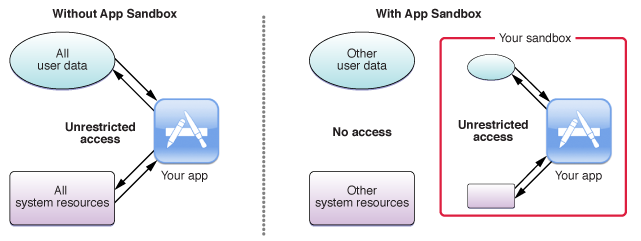
\includegraphics[width=0.9\linewidth]{ios/media/sandboxing.png}
				\caption{Sandboxing unter iOS 
				\cite{IOSSandboxing}}
				\label{fig:sandboxing}
			\end{figure}
			Aufgrund der virtuellen Sperre durch die Sandbox ist es einer App nicht
			möglich Daten anderer Drittanbieter- oder Systemapps anzusprechen. Jede App
			hat ein bei der Installation zugewieses Home-Verzeichnis, in
			welchem Sie ihre Dateien hält. Wenn andere als die eigenen Daten benötigt
			werden, wird dies nur mit vorgeschriebenen APIs vom System ermöglicht. Zu
			Beginn war dies offiziell nicht vorgesehen und so hat sich die
			Entwicklergemeinde selbst einen Weg in Form von \textsl{URL-Schemas}
			gebahnt. Später kam eine weitere Möglichkeit mit dem Nutzen einer
			%TODO: footnote key chain
			gemeinsamen \textsl{Key-Chain} pro \textsl{App Group}
			dazu \cite[S.83]{Banks2015}. Diese App Groups müssen vom Entwickler explizit
			angelegt werden, um anschließend die benötigten Apps darin registrieren zu
			können.
				
		\paragraph{Entitlements}
			Einen weiteren Schutz zur Laufzeit stellen sogenannte \textsl{Entitlements}
			dar, mit denen der Zugriff auf iCloud, Push	Notifications und
			Nutzerinformationen geregelt wird. Da diese digital signiert sind, können Sie
			nicht verändert werden. Entitlements sind Schlüssel-Werte Paare, welche eine
			%TODO: clear this up a little bit more
			Authentifizierung - im Gegensatz zu UNIX Benutzern - ungeachtet der Laufzeit
			zulassen und explizit einer App zugeordnet sind.
			Systemapps und Hintergrundprozesse nutzen diese Berechtigung besonders oft,
			da so verhindert wird, dass der Prozess, welcher das Entitlement gestartet
			hat, mit Root-Rechten laufen muss.
			Zusätzlich verringert dies das Risiko einer ungewollten Rechteerweiterung
			durch einen manipulierten Hintergrundprozess oder einer Systemapp.
		
		\paragraph{ASLR}\label{sec:ios-aslr}
			%TODO: refer to android too
			Für zusätzlichen Laufzeitschutz wurde \textsl{Address space layout
			randomization} \cite[S.1]{iOS4SecurityEvalutaion} ab iOS 4.3 eingeführt. Dies
			weist Programmen zufällige Speicheradressen zu. Somit sollen Angriffe die auf
			Speicherüberläufen basieren verhindert werden \cite[S.131]{Levin2012}. Jedoch
			wird nur der Heap und die Bibliotheken der App durch
			ASLR geschützt, wenn die App nicht mit einer Unterstützung für
			\textsl{Position Independent Executables}\footnote{PIE: Position-Independent
			Executable - Code der, ungeachtet seiner absoluten Adresse im Hauptspeicher,
			ausgeführt werden kann} kompiliert wurde.
			\begin{figure}[h]
				\centering
				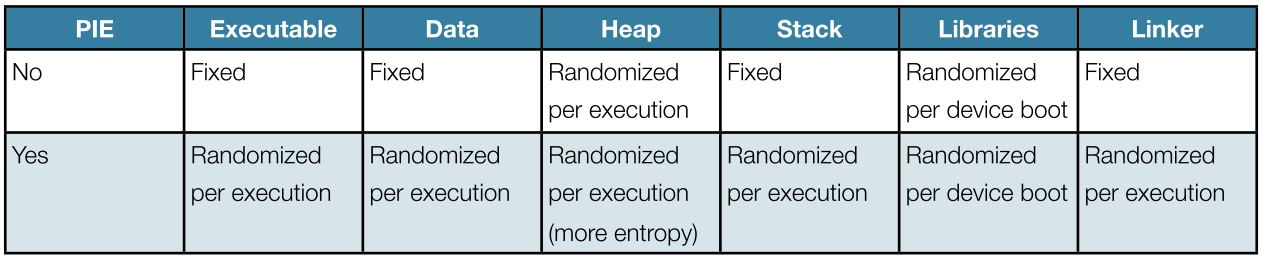
\includegraphics[width=0.9\linewidth]{ios/media/aslr-pie.jpg}
				\caption{ASLR in Abhängigkeit von PIE
				\cite[S.1]{iOS4SecurityEvalutaion}}
				\label{fig:aslr}
			\end{figure}
		
		\paragraph{ARM Never eXecute}
			Mit dem \textsl{NX-Bit} markiert iOS einzelne Speicherseiten entweder mit dem
			\textsl{Code-Flag} oder mit dem \textsl{Data-Flag}. Speicherseiten mit
			Data-Markierung starten einen \textsl{Page-Fault}, wenn ein Programm in
			diesem nicht ausführbaren Speicherbereich versucht eine Adresse auszuführen
			- was bedeuted, dass der Instruction Pointer versucht diesen Bereich
			aufzurufen. Dieser Seitenfehler wird von iOS registriert und damit die
			Ausführung des Programmes unterbunden \cite[S.310]{Levin2012}.